\documentclass[tikz,border=6pt]{standalone}
\usepackage{tikz}
\usetikzlibrary{arrows.meta,positioning,shapes.geometric}

\begin{document}
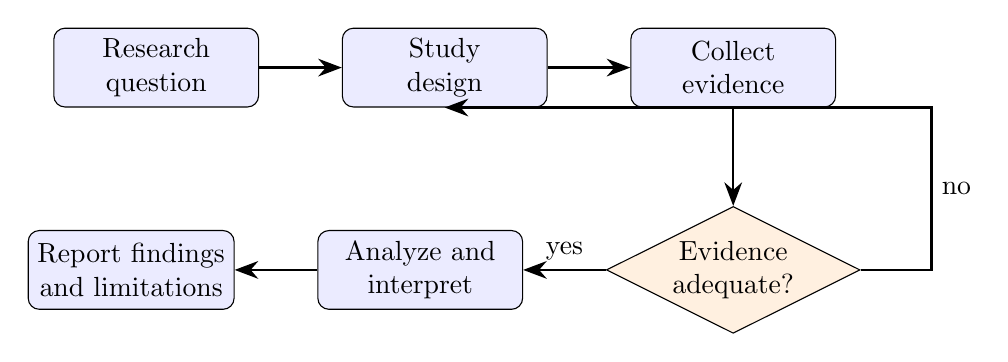
\begin{tikzpicture}[
    node distance=1.25cm and 1.05cm,
    phase/.style={rectangle, rounded corners, draw=black, fill=blue!8,
                 minimum width=2.6cm, minimum height=1cm, align=center},
    decision/.style={diamond, aspect=2, draw=black, fill=orange!12,
                     inner sep=1pt, align=center},
    arrow/.style={-{Stealth[length=3mm]}, thick}
]
    \node[phase] (question) {Research\\question};
    \node[phase, right=of question] (design) {Study\\design};
    \node[phase, right=of design] (collect) {Collect\\evidence};
    \node[decision, below=of collect] (check) {Evidence\\adequate?};
    \node[phase, left=of check] (analyze) {Analyze and\\interpret};
    \node[phase, left=of analyze] (report) {Report findings\\and limitations};

    \draw[arrow] (question) -- (design);
    \draw[arrow] (design) -- (collect);
    \draw[arrow] (collect) -- (check);
    \draw[arrow] (check) -- node[above]{yes} (analyze);
    \draw[arrow] (analyze) -- (report);
    \draw[arrow] (check.east) -- ++(0.9,0) |- node[pos=0.25,right]{no} (design.south);
\end{tikzpicture}
\end{document}
